\documentclass{article}
\usepackage{amsmath}
\usepackage{amssymb}
\usepackage{mathrsfs}
\usepackage{physics}
\usepackage{comment}
\usepackage{mathtools}
\newcommand{\om}{\omega_n}
\newcommand{\adag}{a^\dagger}
\newcommand\Chi{\mathrm{X}}
\newtheorem{problem}{Problem}
\title{Error Mitigation}
\author{Eesh Gupta }
\date{Current Version: March 19, 2020}
\begin{document}
\maketitle
\tableofcontents
\newpage
\section{Introduction}
Isolating physical quantum systems is hard. For this reason, most quantum
systems are considered \textit{open} in the sense that the system
inevitably interacts with its external environment. To illustrate, consider
a qubit represented by 2 discrete states of an electron. Being a charged
particle, that electron is naturally bound to interact with other charged
particles and surrounding electromagnetic fields. This means that the
\textit{environment} can affect the state of the electron as well as the
qubit it represents. These uncontrollable effects are called \textit{noise}
and they can significantly affect our chemistry computations. To understand
the nature of such quantum noise, we will first turn our attentention to
classical noise.
\section{Classical Noise}
Imagine a bit inside a computer hard-drive with external magnetic fields. These
magnetic fields have potential to change the state of the bit with a probability
of let' say \(p\). Let \(i_0, i_1\) be initial probabilities of the bit being
in state 0 and 1 respectively. Similarly, let \(j_1, j_2\) be the new probabilities
after the bit interacts with the magnetic field. Then, we can represent such
\textit{noisy} event as
\[
 \begin{bmatrix}
  j_0 \\
  j_1 \\
 \end{bmatrix}
 =
 \begin{bmatrix}
  1-p &  & p   \\
  p   &  & 1-p \\
 \end{bmatrix}
 \begin{bmatrix}
  i_0 \\
  i_1 \\
 \end{bmatrix}.
\]
\[\begin{bmatrix}
  j_0 \\
  j_1 \\
 \end{bmatrix}
 =
 \begin{bmatrix}
  (1-p)i_0 + pi_1 \\
  pi_0 + (1-p)i_1 \\
 \end{bmatrix}\]
We can make sense of this equation by looking at the equality \(j_0 = (1-p)i_0 + pi_1 \).
Here, \(j_0\) denotes the final probability of the bit being in state 0. If the probability of initial state being 0 is \(i_0\),
then the probability of getting state 0 after interaction is \((1-p)i_0\). In this case,
we multiplied the probability of no-bit-flip  \(1-p\) with \(i_0\). On the other hand, if the probability of initial state being 1
is \(i_1\), then the probability of getting state 0 after interaction is the product of
bit-flip probability \(p\) and \(i_1\). Thus, the probability of getting the final
state of 0 i.e. \(j_0\) is simply the sum of \((1-p)i_0\) and \(pi_1\).
Now, we can write the above equations more succintly as
\[\vec{j} = \hat{E}\vec{i}\]
where \(\hat{E}\) is called the evolution matrix (or the \textit{noise} matrix), and
\(\vec{i}, \vec{j}\) are the initial and final probability distributions respectively.
Then, the final state of the system \(\vec{j}\) is said to be ``linearly'' related to the
initial state of the system \(\vec{i}\).

Note that for the \textit{noise} matrix to describe such a linear transformation, it has
to abide by 2 rules:
\begin{itemize}
  \item \textit{Positivity}: All entries of \(E\) must be non-negative. If \(E\) has
  negative entries, then the vector \(E\vec{q}\) will have negative components i.e.
  negative probabilities. That would be non-sensical.
  \item \textit{Completeness}: The entries in each column of \(E\) must add up to 1.
  Suppose
  \(\vec{i} = \begin{bmatrix}
    x \\
    y \\
  \end{bmatrix}\) and \(
  E = \begin{bmatrix}
    a && c \\
    b && d \\
  \end{bmatrix}\)
  Then
  \[\vec{j} = E\vec{i} = \begin{bmatrix}
    ax + cy \\
    bx + dy \\
  \end{bmatrix}\]
  For \(\vec{i}, \vec{j}\) to be valid probability distribution, their components
  must add up to 1. Then we can assume that \(x+y = 1\), and
  \(ax + cy + bx + dy = 1\) or \((a+b)x + (c+d)y = 1\). For the latter equation
  to be true for any non-trivial inputs \(x, y\) such that \(x+y = 1\),
  both coefficients \(a+b\) and \(c+d\) must be equal to 1. Since these coefficients
  represent the sum of entries of each column of \(E\), we conclude that
  the sum of entries of each column of \(E\) must be equal to 1.
\end{itemize}
\subsection{Markov Process}

Earlier we only looked at one ``noise event''.
Now suppose we have 2 \textit{noisy} gates \(A\) and \(B\). An important
assumption that we can make here is whether gate \(A\) works correctly is
independent of whether gate \(B\) works correctly. That is, the \textit{noisiness}
of gate \(A\) in independent of the \textit{noisiness} of gate B. This assumption
can be \textit{physically reasonable} in cases such as the one where gate \(A\)
and \(B\) are placed a significant distance apart from each other. Then the
process of gate \(A\) and \(B\) being applied in any order is known as Markov
process.

With each noise event being indpendent and being described by a linear transformation,
then the final state after a multiple
noise events is still linearly related to
the initial state.

\section{Quantum Operations}
Quantum Operations offer us tools to understand how quantum states
react to noise. Just as we used a vector of probabilities to
describe initial state and final state, we will use \textit{density
matrices} \(\rho\) to describe initial and final state.
\[\rho \longrightarrow \mathcal{E}(\rho)\]
Here \(\mathcal{E}\) describes a quantum operation. For example, \(\mathcal{E}(\rho)\) could be \(U\rho U^{\dagger}\) where \(U\) is
some unitary operator. Now, before moving onto quantum operations, we
will briefly discuss density matrices and outer products.
There are 3 ways to understand quantum operations: Operator sum representation, physically
motivated axioms and system coupled to environment.
\subsection{Mathematical Interlude}
\subsubsection{Outer Products}
Inner Products such as \(\bra{\phi}\ket{\psi}\) are \textbf{complex numbers}
and describe the \textit{probability amplitude of
the system to \textbf{be} in state \(\phi\) if the system \textbf{is} in
state \(\psi\) }. In contrast, outer products like
\(\ket{\phi}\bra{\psi}\) are \textbf{linear operators} which act on states in a special way. To see such actions, we are going to consider a special case
of outer products: projection operators.

Projection Operators are of the of the form \(\ket{\psi}\bra{\psi}\).
Assume \(\ket{\psi}\) is normalized. When acting on some state \(\ket{A}\), we obtain
\[\ket{\psi}\bra{\psi}   \ket{A} =\bra{\psi}\ket{A}\ket{\psi}.\]
Here the action of projection operator gave us the component of \(\ket{A}\) in the direction of state \(\ket{\psi}\) i.e. the projection of \(\ket{A}\) onto \(\ket{\psi}\).

Here are some properties of projection products:
\begin{enumerate}
  \item Projection operataors are hermitian.
  \item Eigenvector of the projection operator \(\ket{\psi}\bra{\psi}\)
  is \(\ket{\psi}\) itself with an eigenvalue of 1.
  \item Any vector orthogonal \(\ket{\phi}\)to \(\ket{\psi}\) is an eigenvector with an eigenvalue of 0. This is because the term \(\bra{\phi}\ket{\psi} = 0\).
  \item The square of a projection operator \(P\) is \(P\)
  itself. So if \(P = \ket{0}\bra{0}\), then
  \[P^2 = \ket{0}\bra{0}\ket{0}\bra{0} = \ket{0}\bra{0} = P\]
  \item Trace of a projection operator is equal to 1 or
  \[\text{Tr}(\ket{\psi}\bra{\psi}) = \sum_{i = 0}^n \bra{i}\ket{\psi}\bra{\psi}\ket{i} \]
  \[= \sum_{i = 0}^n |\bra{i}\ket{\psi}|^2 = 1\]
  This is true because we are summing over the \textit{shadows of
  \(\ket{\psi}\) in each direction of the Hilbert space defined by
  the basis \(\{i\}\).} Since \(\ket{\psi}\) is of length 1 i.e.
  normalized, the whole sum must be equal to 1.
  \item The sum of all projection operators of a basis is equal to
  identity.
  \[\sum_{i=0}^n \ket{i}\bra{i} = I \]
  This is true because all vectors are eigenvectors of \(\sum_{i=0}^n \ket{i}\bra{i}\) with an eigenvalue of 1. Since this is only true for the identity matrix, the 2 operators are equal to each other.
  \item The expectation value of any observable \(A\) in
  state \(\ket{\psi}\)is given by
  \[\bra{\psi}A\ket{\psi} = \textit{Tr} (\ket{\psi}\bra{\psi}A)\]
  To see why this is true, note that
  \[\textit{Tr} \ket{\psi}\bra{\psi}A = \sum_{i = 0}^n \bra{i}\ket{\psi}\bra{\psi}A\ket{i}\]
  \[=  \sum_{i = 0}^n \bra{\psi}A\ket{i}\bra{i}\ket{\psi}\]
  \[= \bra{\psi}A(\sum_{i = 0}^n \ket{i}\bra{i})\ket{\psi}\]
  \[= \bra{\psi}A I\ket{\psi}\]
  \[= \bra{\psi}A\ket{\psi}\]
  which is the expectation value of A.

\end{enumerate}
\subsubsection{Density Matrices}
In most cases, you will not know the true definite state of a quantum system. Instead
you would be told that the quantum system has \(\lambda_a\) probability of
being in \(\ket{A}\) and \(\lambda_b\) probability of being in \(\ket{B}\).
So how would you package all this information?
Consider the expectation values of some operator L with respect to states
\(\ket{A}\) and \(\ket{B}\):
\[\bra{A}L\ket{A} = Tr{\ket{A}\bra{A}L}\]
\[\bra{B}L\ket{B} = Tr{\ket{B}\bra{B}L}\]
Now accounting for the probabilities, the new expectation value for observable
L becomes
\[\expval{L} =\lambda_A Tr{\ket{A}\bra{A}L} +\lambda_B Tr{\ket{B}\bra{B}L} \]
This ``mixture of states'' becomes more compact if we define
\[\rho = \lambda_A \ket{A}\bra{A} + \lambda_B \ket{B}\bra{B} \]
So,
\[\expval{L} =Tr{\rho L}\]
This quantity \(\rho\) is known as a density matrix or a density operator.
It encodes the probability of the system being in a mix of states. In the
example above, we had more than one state, each given with some associated
probability. This is known as a ``mixed state''. On the other hand, if we
know that our quantum system is definitely in state \(\ket{A}\), our resulting
density operator \(\rho = \ket{A}\bra{A}\) would represent a ``pure state''.

Now, \textit{density matrices} are really \textit{operators} that don't become
matrices until you choose an orthonormal basis. If we choose an orthonomal
basis \(\ket{a}\). Then the matrix representation of \(\rho\) with respect
to this basis is
\[\rho_{a, a'} = \bra{a}\rho\ket{a'}\]
i.e. \(\rho_{a, a'} \) is the entry of the \(a\)'th row and \(a'\)'th
column of the matrix.

Let's choose a special orthonormal basis for the density operator such that
the resulting density matrix is a diagonal matrix i.e. all the elements off the
main diagonal are 0. What we would find is that the sum of the diagonal entries
is 1. Why would that be case? Consider the eigenvectors, \(e_1,
e_2, \ldots, e_n\). Each diagonal element is then an eigenvalue \(\lamda_i\)
of some eigenvector \(\vec{e_i}\)
A special property of density matrices is that the sum of the diagonal entries is 1.
In other words,
\[ \sum_a \bra{a}\rho\ket{a} =\sum_a \rho_{a,a} = 1\]

\(\rho\) (\textit{can be verified easily}).  So if all
the eigenvalues i.e. probabilities are equal, then the density matrix is just proportional to
the unit matrix. What does this mean? That we have absolutely no knowledge
about the system as system is equally likely to be in any of those eigenstates.

 Let's say we wanna convert the expectation value
of observable \(\textbf{L}\) in this representation. Then, we would proceed
as follows:
\[\expval{\textbf{L}} =Tr{\textbf{L}\rho} = \sum_{a'} \bra{a'}\textbf{L}\rho\ket{a'}\]
Suppose we have an identity matrix \(I\) sandwhiched between \(\textbf{L}\)
and \(\rho\). Using the trick \(I = \sum_{a}\ket{a}\bra{a}\) from outer
products,
\[\expval{\textbf{L}} = \sum_{a'} \bra{a'}\textbf{L}\sum_{a}\ket{a}\bra{a}\rho\ket{a'}\]
\[= \sum_{a'}\sum_{a} \bra{a'}\textbf{L}\ket{a}\bra{a}\rho\ket{a'}\]
\[= \sum_{a, a'} L_{a', a}\rho_{a, a'}\]
\subsubsection{Density Matrices and Entanglement}
Alice and Bob each have their own systems. Alice's system can
be in any of the states \(\ket{a}\) and Bob's system can be in any
of the states \(\ket{b}\).
Let's say Alice knows that the state of the combined system is
described the wavefunction \(\psi(a, b)\) where a and b are
discrete variables.
\[\text{state of the system}= \(\ket{\Psi}\) = \sum_{a,b} \psi(a, b)\ket{ab}\]
Suppose Alice wants to do a measure some observable \textbf{L} on her own system,
completely ignoring Bob's system. In other words, we apply an observable
\(\~{\textbf{L}} = \textbf{L}_a\otimes\textbf{I}_b\) on the combined system. The
expectation value \(\~{\textbf{L}}\) is
\[\expval{\~{\textbf{L}}} = \bra{\Psi}\~{\textbf{L}}\ket{\Psi}\]
\[= (\sum_{a',b'} \psi(a', b')\ket{a'b'})\~{\textbf{L}}(\sum_{a,b} \psi(a, b)\ket{ab})\]
\[= \sum_{a, a', b, b'} \psi(a', b')\ket{a'b'}\~{\textbf{L}}\ket{ab}\psi(a, b) \]
Since \(\~{\textbf{L}}\) is just the identity on \(\ket{b}\) and
\(\bra{b'}\ket{b} = 0\) if \(b \neq b'\), all the terms
in the grand summation with \(b \neq b'\) are 0. So getting
rid of those 0 terms, we have
\[\sum_{a, a', b} \psi(a', b)\ket{a'b}{\~\textbf{L}}\ket{ab}\psi(a, b) \]
\[ \sum_{a, a', b} \psi(a', b)\ket{a'}{\textbf{L}}\ket{a}\psi(a, b) \]
\[\sum_{a, a', b} \psi(a', b)L_{a,a'}\psi(a, b) \]
\[\sum_{a, a'} L_{a,a'} \sum_b \psi(a', b)\psi(a, b)\]
Let
\[\rho_{a, a'} = \sum_b \psi(a, b) \psi(a', b) \]
Here \(\rho_{a, a'}\) is known as the reduced density matrix of
subsystem A.










\subsection{Quantum Mechanics Interlude: Measurement}
%%https://inst.eecs.berkeley.edu/~cs191/fa14/lectures/lecture89.pdf
Measurement in quantum mechanics is described by measurement operator \(\{M_m\}\)
where \(m\) denotes the various measurement outcomes. In this section, I will list
some properties of the quantum measurement. To make these properties concrete,
I will assume these operators \(\{M_m\}\) to be projectors. \textit{Why such
assumption?} Projective measurements are simple, ideal and intuitive--and make
explanations a lot easier!

Now suppose we have some initial state \(\ket{\psi}\).
\begin{itemize}
  \item \textit{The probability of observing a measurement outcome \(m\) is
  \(\bra{\psi}{M_m}^{\dagger}M_m\ket{\psi}\).}

  Since \(M_m\) is a projection
  operator, \(M_m\) is hermitian (\(M_m = {M_m}^{\dagger}\)) and \(M_m^2= M_m\).
  Then \(M_m{M_m}^{\dagger}\) is just \(M_m \). So
  \[\bra{\psi}{M_m}^{\dagger}M_m\ket{\psi} = \bra{\psi}M_m\ket{\psi}\]
  Let's say \(\ket{m}\) is the associated eigenvector associated with measurement
  outcome \(m\). Then \(M_m = \ket{m}\bra{m}\). So,
  \[\bra{\psi}\ket{m}\bra{m}\ket{\psi}\]
  which is equal to
  \[|\bra{m}\ket{\psi}|^2\]
  Here, \(\bra{m}\ket{\psi}\) is the probability amplitude of taking
  \(\ket{\psi}\) to the state \(\ket{m}\) or the shadow (i.e. projection) of
  \(\ket{\psi}\) onto the state \(\ket{m}\). From elementary quantum mechanics,
  we know that the square of the norm of such complex number \(|\bra{m}\ket{\psi}|^2\)
  must be the \textit{probability of measuring the system to be in state
  \(\ket{m}\)}.

  Hence, \(\bra{\psi}{M_m}^{\dagger}M_m\ket{\psi}\) is indeed The probability
  of observing a measurement outcome \(m\).

  \item \textit{Completeness Relation: \(\sum_m {M_m}^{\dagger}M_m = I\).}

  Recall from above that \(M_m{M_m}^{\dagger}= M_m \). Then
  \[\sum_m {M_m}^{\dagger}M_m = \sum_m M_m  \]
  And
  \[\sum_m M_m = \sum_m \ket{m}\bra{m}\]
  Since we are summing over all the measurement outcomes, we are also
  summing over all the projectors of some basis. So, as noted in
  the ``Outer-products'' section,
   \[\sum_m \ket{m}\bra{m} = I\]
  Another way to look at the completeness relation is that it implies that
  \(\sum_m p(m) = 1\) i.e. the sum of probabilities of measuring
  all outcomes is 1.


  \item \textit{The state of the system immediately followed by measurement of
  outcome \(m\) is
  \[\ket{\psi} = \frac{M_m \ket{\psi}}
  {\sqrt{\bra{\psi}{M_m}^{\dagger}M_m\ket{\psi}}}.\]}
  Let's take it apart. The numerator is
  \[M_m \ket{\psi} = \ket{m}\bra{m}\ket{\psi} = \alpha\ket{m}\]
  Here \(\alpha\) is the \textit{probability amplitude of being in state
  \(\ket{\psi}\) if in state \(\ket{m}\).}
  On the othe hand, the denomiator is
  \[\sqrt{\bra{\psi}{M_m}^{\dagger}M_m\ket{\psi}} =
  \sqrt{\bra{\psi}M_m\ket{\psi}}\]
  \[= \sqrt{\bra{\psi}\ket{m}\bra{m}\ket{\psi}}\]
  \[= \sqrt{|\alpha|^2} = |\alpha|\]
  So the fraction becomes
  \[\frac{\alpha\ket{m}}{|\alpha|}\]
  Here \(\frac{\alpha}{|\alpha|} = e^{i\phi}\) for some \(\phi \in [0,2\pi)\).
  Since global phases aren't of much importance, we can equivalently say
  that the final state is just \(\ket{m}\). This makes sense because
  after ``observing '' the outcome \(m\), the whole state \(\ket{\psi}\)
  ``collapses'' to the state \(\ket{m}\).

\end{itemize}
\subsection{Basic Operations}
\subsubsection{Unitary Evolution}
%%\textit{Parallels between evolution of pure states and evolution of density matrices.}
\textit{Under unitrary transformations, density matrices \(\rho\)
evolve as \(U\rho U^{\dagger}\)}

If normal ket states evolve under unitary transformations as
\[\ket{\psi} \longrightarrow U\ket{\psi}\]
Then, its hermitian conjugate evolves as
\[\bra{\psi} \longrightarrow \bra{\psi}U^{\dagger}\]


So ince \(\rho\) is combination of both states i.e. \(\rho = \ket{\psi}\bra{\psi}\), then \(\rho\) evolves as
\[\ket{\psi}\bra{\psi} \longrightarrow U\ket{\psi}\bra{\psi}U^{\dagger} \]
So,
\[\rho \longrightarrow U\rho U^{\dagger} \equiv \mathcal{E}(\rho) \]

\subsubsection{Measurement}
% How this relates to qm section
If the measurement operator \(M_m\) describes the unitary transformation of density matrix \(\rho\), we know from
the previous section that the resulting state would be
\(M_m\rho M_m^{\dagger}\). To see an example of this
in action, suppose that we are making simple projective
measurements on a system which is in a pure state. So
\(M_m = \ket{m}\bra{m}\) and \(\rho = \ket{\psi}\bra{\psi}\).
Also recall that \(M_m\) is hermitian i.e. \(M_m = M_m^{\dagger}\). Then,
\[M_m\rho M_m^{\dagger} = \ket{m}\bra{m}\ket{\psi}\bra{\psi}\ket{m}\bra{m}\]
\[= \ket{m}\alpha\alpha^{\star}\bra{m}\]
\[= \ket{m}|\alpha|^2\bra{m}\]
where \(\alpha = \bra{m}\ket{\psi}\) is the probability amplitude of
the system \textbf{being} in \(\ket{m}\)
if the system \textbf{is} in state \(\ket{\psi}\) . Then \(|\alpha|^2\)
is just real number denoting the probability of measuring the system to be in state
\(\ket{m}\). So finally
\[M_m\rho M_m^{\dagger} = |\alpha|^2\ket{m}\bra{m}\]
To get rid of the coefficient \(|\alpha|^2\), we introduce another term
\(Tr(M_m\rho M_m^{\dagger})\). We will now verify that \(Tr(M_m\rho M_m^{\dagger})\)
is indeed equal to \(|\alpha|^2\).
\[Tr(M_m\rho M_m^{\dagger}) = \sum_i \bra{i}M_m\ket{\psi}\bra{\psi}M_m^{\dagger}\ket{i}\]
\[= \sum_i \bra{\psi}M_m^{\dagger}\ket{i}\bra{i}M_m\ket{\psi}\]
\[= \bra{\psi}M_m^{\dagger}(\sum_i\ket{i}\bra{i})M_m\ket{\psi}\]
\[= \bra{\psi}M_m^{\dagger}M_m\ket{\psi}\]
As noted in the quantum mechanics interlude, \(M_m^{\dagger}M_m=M_m \). So,
\[= \bra{\psi}M_m\ket{\psi}\]
\[= \bra{\psi}\ket{m}\bra{m}\ket{\psi}\]
\[= \alpha^{\star}\alpha\]
So,
\[Tr(M_m\rho M_m^{\dagger}) = |\alpha|^2\]
Thus, using this term to get rid of the coefficient from the state \(M_m\rho M_m^{\dagger} = |\alpha|^2\ket{m}\bra{m}\),
the final state after the measurement becomes
\[\frac{M_m\rho M_m^{\dagger}}{Tr(M_m\rho M_m^{\dagger})}\]
If we make  \(\mathcal{E}_m(\rho) = M_m\rho M_m^{\dagger}\), then the
above expression simplifies to
\[\frac{\mathcal{E}_m(\rho)}{Tr \mathcal{E}_m(p)}\]
where \(Tr \mathcal{E}_m(p)\) is the probability of measuring the system to
be in state \(\ket{m}\).


\subsection{Systems Coupled to Environment}

Closed Systems can be easily described by unitary transformations as shown
in figure 1.
\begin{figure}[!htb]
	\centering
	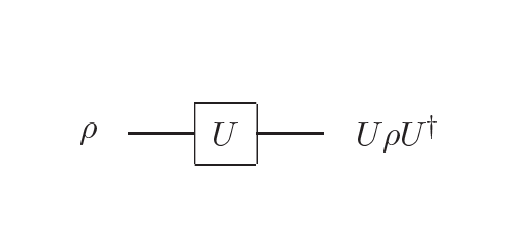
\includegraphics[width=0.95\textwidth]{img/SystemPure1.png}
	\caption{The input state \(\rho\) is trasnformed into the output
  state \(U\rho U^{\dagger}\).}
	\label{}
\end{figure}
However, to model open system, we consider the closed system of
the system and environment
\begin{figure}[!htb]
	\centering
	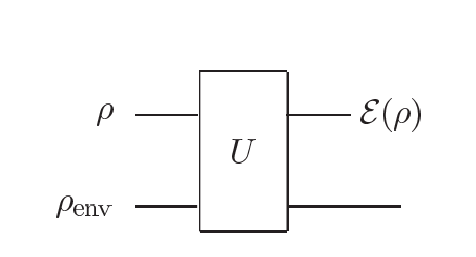
\includegraphics[width=0.95\textwidth]{img/opensystem.png}
	\caption{Closed system consisting of the system of interest
  and the environment}
	\label{}
\end{figure}
Suppose the system-environment system starts out in some product state
\(\rho \otimes \rho_{env}\). (why such assumption? Are the experimentalists controlling the
qubit so it doesn't further interact with environment?) Then after the
unitary transformation, the combined system is in state
 \(U(\rho \otimes \rho_{env})U^{\dagger}\).
 To get rid of the environment state \(\rho_{env}\) in order to obtain
 only the state of the system of interest after the unitary transformation,
 we perform a partial trace over the environment state. So, the final state of our system of interest is
 \[\mathcal{E}(\rho) = Tr_{env}(U(\rho \otimes \rho_{env})U^{\dagger})\]
%http://www.quantum.umb.edu/Jacobs/QMT/QMT_AppendixA.pdf

 \textit{Why partial trace?} Suppose you have some product state
 \(\rho_{A} \otimes \rho_{B}\). To isolate the state \(\rho_A\) from the
 product state, at least mathematically, we need to get rid of \(\rho_B\).
 Recall from the property of density matrices that \(Tr \rho = 1\). So tracing
 over B, we have
 \[Tr_B (\rho_{A} \otimes \rho_{B}) = \rho_{A} \otimes Tr_B \rho_{B} = \rho_{A}\]
 Intuitively, we are averaging over the states of the environment to isolate
 the state of system \(A\).

\subsection{Operator Sum Representation}
Assume the basis \({e_k}\) for the \(\rho_{env}\) and let \(\rho_{env}\) be a
pure state equal to the projector \(\ket{e_0}\bra{e_0}\). Then we can
expand the expression
\[Tr_{env}(U(\rho_A \otimes \rho_{env})U^{\dagger}) \]
as
\[\sum_k (\mathbb{I}_A \otimes \bra{e_k})U(\rho_A \otimes \ket{e_0}\bra{e_0})U^{\dagger}(\mathbb{I}_A \otimes \ket{e_k})\]
Now the expression
\[\rho_A \otimes \ket{e_0}\bra{e_0} = (\rho_A \otimes \mathbb{I}_e)(\mathbb{I}_A \otimes\ket{e_0})(\mathbb{I}_A \otimes \bra{e_0})\]
where the subexpression
\[(\rho_A \otimes \mathbb{I}_e)(\mathbb{I}_A \otimes\ket{e_0}) = (\rho_A\mathbb{I}_A) \otimes (\mathbb{I}_e\ket{e_0})\]
Since the product \(\rho_A\mathbb{I}_A\) is commutative and \(\mathbb{I}_e\ket{e_0} = \ket{e_0}\),
we have
\[ = (\mathbb{I}_A\rho_A) \otimes (\ket{e_0}\cdot 1)\]
\[ = (\mathbb{I}_A \otimes \ket{e_0})(\rho_A \otimes 1)\]
So, \[(\rho_A \otimes \mathbb{I}_e)(\mathbb{I}_A \otimes\ket{e_0}) = (\mathbb{I}_A \otimes \ket{e_0})\rho_A\]
Then plugging this subexpression back into the former expression, we have
\[\rho_A \otimes \ket{e_0}\bra{e_0} = (\mathbb{I}_A \otimes \ket{e_0})\rho_A(\mathbb{I}_A \otimes \bra{e_0})\]
So, the equation for \[\mathcal{E}(p)\] becomes
\[\mathcal{E}(p) = \sum_k (\mathbb{I}_A \otimes \bra{e_k})U(\mathbb{I}_A \otimes \ket{e_0})\rho_A(\mathbb{I}_A \otimes \bra{e_0})U^{\dagger}(\mathbb{I}_A \otimes \ket{e_k})\]
\[\mathcal{E}(p) = \sum_k E_k \rho_A E^{\dagger}_k\]
where
\[E_k = (\mathbb{I}_A \otimes \bra{e_k})U(\mathbb{I}_A \otimes \ket{e_0})\]
\[E^{\dagger}_k = (\mathbb{I}_A \otimes \bra{e_0})U^{\dagger}(\mathbb{I}_A \otimes \ket{e_k})\]
Environment starts in pure state. Operators act on principal system's Hilbert space
alone.
Properties of \(E_k\):
\begin{enumerate}
  \item Completeness
    Since \(\mathcal{E}(p)\) is a density matrix representing resultant state of
    system \(A\), then
    \[Tr\mathcal{E}(p) = 1\]
    So,
    \[Tr(\sum_k E_k E^{\dagger}_k \rho) = 1\]

    \textit{What's Happening?} As of now, we have extracted state of principal system \(\mathcal{E}(\rho)\)
    from the evolved product state of principal system and environment \(U(\rho_A \otimes \rho_{env})U^{\dagger}\). Here we verify that if \(\mathcal{E}(\rho)\) is made up of
    different states, then the probabilities corresponding to all those states add up to one.

  \item Trace Preserving

  Looking carefully at the completeness relation, we see that
  \[Tr\mathcal{E}(p) = Tr (\sum_k E_k E^{\dagger}_k) = 1\]
  is true for arbitrary state \(\rho\).
\end{enumerate}
\subsection*{Importance of Operator Sum Representation}
\textit{not explicitly consider properties of environment}

\subsubsection*{Measurement}
In this subsection, we will solve exercise 8.4 of Nielsen and Chuang.
\begin{problem}
  Suppose you have a single qubit
  principal system in some state \(\rho\) and environment
  in pure state \(\ket{0}\bra{0}\). Given the unitary transformation
  \[U = P_0 \otimes I  + P_1 \otimes X\]
  where \(P_0 = \ket{0}\bra{0}\), \(P_1 = \ket{1}\bra{1}\) act on the
  the principal system and the pauli matrix \(X\) acts on the environment,
  suppose the system ``interacts with the environment through the transform"
  (???? \textit{wierd unclear phrasing alert}) \(U\). Give the quantum
  operation for this process in the operator-sum representation.
\end{problem}

\textit{Solution} Recall that a quantum operation is described by
\[\mathcal{E}(\rho) = Tr_{env}(U(\rho \otimes \rho_{env})U^{\dagger})\]
Now the basis for environment will be the usual computation basis as we are
assuming all systems to be single qubit. So,
\[\mathcal{E}(\rho) = \sum_{k=0}^{1}(I \otimes \bra{k})(U(\rho \otimes \ket{0}\bra{0})U^{\dagger})(I \otimes \ket{k})\]
In the previous section, we saw that
\[\rho \otimes \ket{0}\bra{0} = (I\otimes \ket{0})\rho(I \otimes \bra{0})\]
So,
\[\mathcal{E}(\rho) = \sum_{k=0}^{1}(I \otimes \bra{k})U(I\otimes \ket{0})\rho(I \otimes \bra{0})U^{\dagger}(I \otimes \ket{k})\]
Now let's simplify smaller subexpressions,
\[ (P_0 \otimes I  + P_1 \otimes X)(I\otimes \ket{0})\]
\begin{equation} \label{eq1}
\begin{split}
 U(I\otimes \ket{0}) &= (P_0 \otimes I  + P_1 \otimes X)(I\otimes \ket{0})\\
 &= (P_0 \otimes I)(I\otimes \ket{0}) + (P_1 \otimes X)(I\otimes \ket{0}) \\
 &= P_0 \otimes \ket{0} + P_1 \otimes \ket{1}\\
\end{split}
\end{equation}
Then the following subexpression can be simplified as
\begin{equation} \label{eq2}
\begin{split}
 (I\otimes \bra{0})U(I\otimes \ket{0}) &= (I\otimes \bra{0})(P_0 \otimes \ket{0} + P_1 \otimes \ket{1})\\
 &= P_0 \otimes \bra{0}\ket{0} + P_1 \otimes \bra{0}\ket{1}\\
 &= P_0 \otimes 1 + P_1 \otimes 0\\
 &= P_0
\end{split}
\end{equation}
Similarly we can show that
\[(I\otimes \bra{1})U(I\otimes \ket{0}) = P_1\]
\[(I\otimes \bra{0})U(I\otimes \ket{1}) = P_1\]
So the quantum operation \(\mathcal{E}(\rho)\) can be simplified as
\[\mathcal{E}(\rho) = P_0 \rho P_0 + P_1 \rho P_1\]
\[\mathcal{E}(\rho) = \rho\]
\textit{need to verify that last step}
\subsubsection*{Spin Flips}
\subsubsection*{Composition of quantum operations}
\subsubsection*{Physical Interpretation of Operator Sum Representation}
Discuss quantum channels and how it relates to classical information
theory.
\subsubsection*{Measurement and Operator Sum Representation}
Given a description of open quantum system, how do we determine its
operator sum representation to decribe its dynamics?
\subsubsection*{System environment models for any operator sum representation}
Given a set of operators \(\{E_k\}\) is there some reasonalble modell
environmental system and dynamics?
\subsubsection*{Mocking up a quantum operation}

\subsection{Physically Motivated Axioms}
some axioms a map has to follow in order to have operator-sum
representation
\begin{enumerate}
  \item \(0\leq \textit{tr} [\mathcal{E}(\rho)]\leq 1\) for any \(\rho\).
  \item \(\mathcal{E}(\sum_{i}p_i\rho_i) = \sum_{i}p_i\mathcal{E}(\rho_i)\).
  \item \(\mathcal{E}\) is a completely positive map.
\end{enumerate}
\section{Examples of Quantum Noise and Quantum Operations}
In the following sections, we will explore how quantum noise deforms the state space
of a single qubit. That is, after some noise operation \(\mathcal{E}\), we will find
certain states changed and other untouched. However, even if \(\mathcal{E}\) \textit{can}
change the state of qubit, it does so with some probability \(p\). So if the
initial state of our single qubit is given by \(\rho\), then we expect \(\mathcal{E}\)
to act as follows
\[ \rho \longrightarrow^{\mathcal{E}} (1-p)\rho + p\mathcal{N}(\rho) \]
where \(\mathcal{N} (\rho)\) is some unitary operation on \(\rho\), deforming
the state. We first begin with a mathematical interlude on bloch spheres and
density matrices. Then we explore ``deforming'' operations \(\mathcal{N}\).

\subsection{Mathematical Interlude: Bloch Spheres and Density Matrices}
\subsubsection{Bloch Sphere Representation of a qubit }
Recall that the state of a single qubit can be specified in terms of
complex number \(\alpha, \beta\) as
\[\ket{\psi} = \alpha\ket{0} + \beta\ket{1}. \]
where \(|\alpha|^2 + |\beta|^2 = 1\).
Since each complex number requires 2 real parameters \(\alpha = \underline{a} +
\underline{b}i\), it seems
that the state \(\ket{\psi}\) will require 4 real parameters. However, if we
 express \(\alpha, \beta\) as
\[\alpha = r_\alpha e^{i\phi_{\alpha}} \text{ and }  \beta = r_\beta e^{i\phi_{\beta}}\]
where \(r_\alpha, r_\beta,\phi_{\alpha}, \phi_{\beta} \in \mathbb{R}\), then
we can extract a global phase factor from \(\ket{\psi}\) as follows:
\[\ket{\psi} = r_\alpha e^{i\phi_{\alpha}}\ket{0} + r_\beta e^{i\phi_{\beta}}\ket{1}\]
\[\ket{\psi} = e^{i\phi_{\alpha}}(r_\alpha\ket{0} + r_\beta e^{i(\phi_{\beta} - \phi_{\alpha})}\ket{1})\]
\[\ket{\psi} = e^{i\phi_{\alpha}}(r_\alpha\ket{0} + r_\beta e^{i\phi}\ket{1})\]
Here \(\phi = \phi_{\beta} - \phi_{\alpha}\) and \(e^{i\phi_{\alpha}}\) is the global
phase factor. Since the global phase factor does not really affect the observables,
we will ignore that term. That leaves us with 3 real parameters: \(r_\alpha, r_\beta \text{ and }\phi\).
Recognizing that \(|\alpha|^2 + |\beta|^2 = 1\) implies \(|r_\alpha|^2 + |r_\beta|^2 = 1\), it
is possible to get rid of another parameter by making the following substitutions
\[r_\alpha = \cos(\frac{\theta}{2}) \text{ and } r_\beta = \sin(\frac{\theta}{2})  \]
Thus we have,
\[\ket{\psi} = \cos(\frac{\theta}{2})\ket{0} + e^{i\phi}\sin(\frac{\theta}{2})\ket{1}\]
where \(0 \leq \theta \leq pi\) and \(0 \leq \phi < 2pi\). So the state of a single
qubit only requires 2 parameters. This has a nice geometrical interpretation
in terms of a unit sphere.
\begin{figure}[!htb]
	\centering
	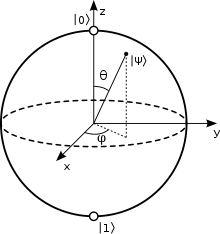
\includegraphics[width=0.5\textwidth]{img/bloch_sphere.png}
	\caption{Wikipedia's Bloch Sphere}
	\label{}
\end{figure}
Now each pure state has an associated bloch vector
\(\vec{r} = (x,y,z) = (\sin\theta \cos\phi,\sin\theta \sin\phi, \cos\theta )\)
Note that \(|r|^2 = 1\) since this is a bloch vector for a pure state. This is so
because pure states lie on the surface of the bloch sphere. It is then natural to
ask geometrical interpreation of a mixed state. To answer that question, we will
first show how a density matrix of some pure state
\(\ket{\psi} = \cos(\frac{\theta}{2})\ket{0} + e^{i\phi}\sin(\frac{\theta}{2})\ket{1}\) relates to its
bloch vector \(\vec{r}\). Recall that
\[\ket{0} = \begin{pmatrix}
  1\\0
\end{pmatrix}
\text{ and }
\ket{1} = \begin{pmatrix}
  0\\1
\end{pmatrix}\]
So, \[\ket{\psi} = \begin{pmatrix}
  \cos(\frac{\theta}{2}) \\
  e^{i\phi}\sin(\frac{\theta}{2})
\end{pmatrix}\]
Then the density matrix \(\rho = \ket{\psi}\bra{\psi}\) can be expressed as
\[\rho = \begin{pmatrix}
  \cos(\frac{\theta}{2})^2 & e^{-i\phi}\sin(\frac{\theta}{2})\cos(\frac{\theta}{2})\\
  e^{i\phi}\sin(\frac{\theta}{2})\cos(\frac{\theta}{2}) & \sin(\frac{\theta}{2})^2
\end{pmatrix}\]
Using some nice double angle trig identities and expanding \(e^{i\phi}\), we simplify the above matrix as follows
\[\rho = \frac{1}{2}\begin{pmatrix}
  1+ \cos(\theta)  & \sin\theta\cos\phi - i\sin\theta\sin\phi\\
  \sin\theta\cos\phi + i\sin\theta\sin\phi & 1-\cos\theta
\end{pmatrix}\]
Now we will convert spherical coordinates into rectangular coordinates as follows
\[x= \sin\theta\cos\phi\]
\[y = \sin\theta\sin\phi\]
\[z = \cos\theta\]
Thus, \(\rho\) now becomes
\[\rho = \begin{pmatrix}
  1 + z & x-iy\\
  x+iy & 1-z
\end{pmatrix}\]
which can be expressed in terms of the pauli matrices as
\[\rho = \frac{1}{2}(\begin{pmatrix}
  1 & 0 \\
  0 & 1
\end{pmatrix} +
x\begin{pmatrix}
  0 & 1 \\
  1 & 0
\end{pmatrix} +
y\begin{pmatrix}
  0 & -i \\
  i & 0
\end{pmatrix} +
z\begin{pmatrix}
  1 & 0 \\0 & -1
\end{pmatrix})\]
Thus, we have
\[\rho = \frac{I + \vec{r}\dot\vec{\sigma}}{2}\]
for which \(\vec{\sigma} = (\sigma_x, \sigma_y, \sigma_z)\)
\subsection{Bit Flip and Phase Flip Channels}
\subsection{Depolarizing Channel}
\subsection{Amplitude Damping}
\subsection{Phase Damping}


\section{Error Mitigation}
\subsection{Extrapolation}
Intentionally increasing dominant error rate by some factor and
using that to determine error free result.
\subsubsection{Richardson's Approach}
\subsection{Probabilistic Error Cancellation}
\textit{Cancelling errors by resampling randomized circuits
according to quasi probability distributions ?!?!??}
Requires full knowledge of the noise model associated with each gate. This
could be obtained from wither process tomography or combo of gate set and
process tomography.

We are dealing with markovian noise here which means maps must be
trace preserving and completely positive.
\subsection{Quantum Subspace Expansion}

\subsection{Other Methods}
\section{References}


\end{document}
